\documentclass[main.tex]{subfiles}

\begin{document}

%\end{comment}
\paraAmbos

\chapter{Polinômios e afins}

%\end{comment}
\paraAlunos

\section{Apresentação}

Polinômios são expressões algébricas extremamente versáteis e com propriedades que os tornam boas opções para diversas aplicações. Ao longo da disciplina de Cálculo você notará que a maioria dos conceitos e teoremas será introduzida através de exemplos envolvendo polinômios. Isso ocorre pela simplicidade das funções polinomiais em comparação com outros tipos de função, pelo menos no contexto dessa disciplina.

Ao longo do seu Ensino Médio você deve ter estudado polinômios em diversos momentos diferentes: equações do primeiro e do segundo grau, fatoração, funções afim e quadrática e talvez até mesmo alguns tópicos sobre polinômios de graus maiores.

Neste capítulo, vamos revistar alguns desses tópicos pensando nos usos que você fará deles em Cálculo e para ter certeza de que você tem fluência com as habilidades mais fundamentais deste tópico.

\newpage

\section{Pré-requisitos e Auto-avaliação inicial}

Os pré-requisitos para este capítulo são:
\begin{itemize}
 \item Resolução de equações do segundo grau;
 \item Produto de binômios.
\end{itemize}

Esses tópicos não serão cobertos durante as atividades de tutoria. Se você acha que não sabe o suficiente sobre algum deles, sugerimos que se procure material de apoio antes de começar a resolver as questões desse capítulo.

Antes de começar, indique o quanto você acha que sabe sobre os seguintes itens:

\begin{center}
 \begin{tabular}{|p{25mm}||p{10mm}|p{10mm}|p{10mm}|p{10mm}|} 
 \hline
   & Nada & Muito pouco & Noções gerais & Muito\\
 \hline
 Fatoração de polinômios &  &  &  &  \\ 
 \hline
 Soma de frações com incógnitas &  &  &  &  \\
 \hline
 Funções racionais &  &  &  &  \\
 \hline
\end{tabular}
\end{center}

%\end{comment}
\paraAmbos

\section{Questões diagnósticas}

\begin{diagnostico}
Fatore a expressão algébrica $$3x^2-12x-36$$.
\end{diagnostico}
  
\begin{diagnostico}
Faça a soma $$\frac{2}{x}+\frac{3}{x-1}$$.
\end{diagnostico}

%\end{comment}
\paraTutores
\subsection{Gabarito}

1) $3(x-6)(x+2)$, 2) $(5x-2)/(x^2-x)$.

\section{Quadro de orientação}

\begin{center}
 \begin{tabular}{|c c c c |c|} 
 \hline
 1A & 1B & 1C & 1D & Onde começar\\
 \hline
 C & E & E & E & Questão 2 \\ 
 \hline
 C & C & E & E & Questão 3 \\ 
 \hline
 C & C & C & E & Questão 7 \\ 
 \hline
 C & C & C & C & Questão 8 \\ 
 \hline
\end{tabular}
\end{center}

%\end{comment}
\paraAmbos

\newpage

\section{Questões}

Lembre-se de checar com seu tutor em qual questão você deve começar.

%\end{comment}
\paraTutores

\subsection{Comentários iniciais}

Nesta seção, serão trabalhados conteúdos relacionados principalmente à manipulação algébrica de polinômios e frações algébricas e, nas últimas questões, acerca de funções que envolvam estes elementos. O objetivo é promover a fluência dos estudantes com algumas manipulações algébricas recorrentes nas disciplinas básicas de matemática focando em expressões que são comuns na disciplina de Cálculo Diferencial e Integral. Os principais conceitos abordados são

\begin{itemize}
 \item Fatoração de expressões quadráticas;
 \item Soma de frações algébricas;
 \item Resolução de equações envolvendo frações algébricas;
 \item Introdução à funções racionais;
\end{itemize}

No início, este capítulo propõe questões que tentam promover a fluência com procedimentos considerados fundamentais, como obtenção de raízes de equações quadráticas, fatoração e soma de frações algébricas. Nessa etapa, é importante que os alunos consigam resolver as questões sem cometer muitos erros procedimentais. Se algum estudante estiver cometendo-os, sugira mais questões semelhantes antes de deixá-lo avançar.

No final, o capítulo se torna mais conceitual e é importante que não haja pressa e que os estudantes resolvam as questões buscando entender o que estão fazendo.

%\end{comment}
\paraAmbos

\subsection*{Equações quadráticas}

As equações quadráticas podem ser apresentadas em vários formatos diferentes, cada um deles com suas vantagens e desvantagens. 

\begin{questao}
\notaTutor{Espera-se que os estudantes não tenham dificuldades com essa questão, mas certifique-se de que eles leram a discussão após a questão.} As equações quadráticas abaixo estão apresentadas em três formatos diferentes. Resolva cada uma delas usando método que lhe parecer mais adequado.
\begin{enumerate}[a)]
\item $x^2-2x-15=0$
\item $(x-5)(x+3)=0$
\item $(x-1)^2-16=0$
\end{enumerate}
\end{questao}

\begin{gabarito}
	\begin{gabaritoQuestao}
		a) $x=5$ e $x=-3$, b) $x=5$ e $x=-3$, c) $x=5$ e $x=-3$.
	\end{gabaritoQuestao}
\end{gabarito}

Você deve ter obtido as mesmas raízes para as três equações. Isso ocorreu porque, na verdade, as três equações são a mesma equação apresentada de forma diferente.

A primeira forma, chamada de desenvolvida, é a mais comum e facilita a aplicação da forma de Bhaskara. Note que apesar da fórmula de Bháskara te dar as raízes após alguns cálculos, não é possível identificá-las diretamente apenas olhando para a equação.

A segunda forma é chamada de fatorada e apesar de demandar algumas manipulações algérbicas para permitir o uso da fórmula de Bhaskara, isso não é necessário, pois as raízes podem ser identificadas na expressão algébrica dada. Isso ocorre porque a forma fatorada apresenta a equação como um produto de fatores, $(x-5)(x+3)$ nesse caso, igualado a zero. Como um produto so é igual a zero se um dos fatores for igual a zero, podemos resolver $(x-5)=0$ e $(x+3)=0$ para obter as soluções da equação.

A terceira forma é bem pouco comum, mas também permite a resolução sem o uso da fórmula de Bháskara. Se você usou a fórmula para resolvê-la cheque se algum colega resolveu sem usá-la ou chame o seu tutor para que ele lhe mostre como.

\subsection*{A forma fatorada}

A grande vantagem da forma fatorada está no fato de ela simplificar a equação: uma equação que originalmente era de segundo grau (envolvia a incógnita ao quadrado) foi transformada em uma produto de fatores que são de primeiro grau (nada de quadrados neles), essa transformação simplifica diversas manipulações que podem ser feitas na expressão. Como vimos acima, facilita inclusive a identificação de raízes.

\begin{questao}
Obtenha as raízes das equações abaixo.
\begin{enumerate}[a)]
\item $(x+2)(x-1)=0$
\item $(x-\frac{2}{3})(2x-4)=0$
\item $5(x+1)(2x-1)=0$
\item $x(6-2x)=0$
\item $-3(x+\sqrt{5})(2x-\sqrt{12})=0$
\end{enumerate}
\end{questao}

\begin{gabarito}
	\begin{gabaritoQuestao}
        a) $x=-2$ e $x=1$, b) $x=2/3$ e $x=1$, c) $x=-1$ e $x=1/2$, d) $x=0$ e $x=3$, e) $x=-\sqrt{5}$ e $x=\sqrt{3}$.
	\end{gabaritoQuestao}
\end{gabarito}

%\end{comment}
\paraTutores

Certifique-se de que os estudantes compreenderam o princípio de igualar os fatores multiplicado a zero caso a equação esteja igualada a zero. Você pode, inclusive, propor a equação $x^2+2x=-1$ para ver se eles notam que esse método não pode ser usado nesse caso.

Uma das raízes do último item envolve uma raiz que pode ser simplificada.

%\end{comment}
\paraAmbos

\begin{reflita}
Com base no que foi visto até este ponto:
\begin{enumerate}[a)]
\item Crie uma equação na forma fatorada e na forma desenvolvida que tenha raízes iguais a $3$ e $4$.
\item Cheque com seus colegas se eles criaram a mesma equação.
\item Crie uma outra equação, diferente da criada no item a, mas que tenha as mesmas raízes.
\end{enumerate}
\end{reflita}

%\end{comment}
\paraTutores

A intenção aqui é salientar o papel da constante ao rescrevermos uma expressão na forma fatorada. Se os estduantes estiverem com dificuldade peça que chequem as raízes de $x^2-7x+10$ e $3x^2-21x+30$.

%\end{comment}
\paraAmbos

\subsection*{Fatoração}

Com as questões anteriores, você já deve ter chegado a um método que lhe permitiria transformar uma expressão do tipo $ax^2+bx+c$ em outra expressão equivalente na forma $a(x-r_1)(x-r_2)$, mas vejamos como seria esse processo para o caso $2x^2+8x+6=0$.

Primeiro, obtemos as raízes de $2x^2+8x+6=0$ usando a fórmula de Bhaskara: $-1$ e $-3$. Agora, escrevemos uma expressão fatorada que tenha essas mesmas raízes: $(x+1)(x+3)$. Ainda falta um passo: note que se desenvolvemos o produto em $(x+1)(x+3)$ obtemos $x^2+4x+3$, que não é igual à expressão inicial. O que nos falta é multiplicar a expressão fatorada por $2$, obtendo $2(x+1)(x+3)$.

Note que esse último passo não altera as raízes e faz com que cheguemos exatamente na expressão dada originalmente se desenvolvermos o produto.

Use essa abordagem para resolver a próxima questão.

\begin{questao}
Fatore as expressões abaixo.
\begin{enumerate}[a)]
\item $x^2-4x+3$
\item $3x^2+9x+6$
\item $\frac{x^2}{2}+2x-16$
\item $5x^2-20$
\item $x^2+6x$
\end{enumerate}
\end{questao}

\begin{gabarito}
	\begin{gabaritoQuestao}
		a) $(x-3)(x-1)$, b) $(x+2)(x+1)$, c) $(x+8)(x-4)$, d) $5(x+2)(x-2)$, e) $x(x+6)$,
	\end{gabaritoQuestao}
\end{gabarito}

%\end{comment}
\paraTutores

Essa questão encerra a primeira parte detse capítulo. Se os estudantes estiverem com dificuldades, crie mais itens como estes para que eles resolvam antes de seguir para a próxima questão, pois ela introduzirá novos conceitos e procedimentos. Algumas sugestões: $x^2+3x+2$, $x^2+4x-5$, $2x^2-4x-2$, $6x^2-4x$, $5x^2-80$ e $15+2x-x^2$.

%\end{comment}
\paraAmbos

\subsection*{Frações}

O próximo passo deste capítulo é aplicar o que vimos até aqui em expressões envolvendo frações com incógnitas no numerador e denominador, mas para isso vamos relembrar como fazer a soma de duas frações simples: $\frac{2}{5}+\frac{3}{7}$.

$$
\frac{2}{5} + \frac{3}{7} = \frac{7 \cdot 2}{7 \cdot 5} + \frac{5 \cdot 3}{5 \cdot 7} = \frac{7 \cdot 2 + 5 \cdot 3}{7 \cdot 5} = \frac{14 + 15}{35} = \frac{29}{35}
$$

Se usarmos frações que envolvam expressões um pouco mais complicadas, na verdade, nada deve mudar. Por exemplo, se fizermos a eguinte soma: $\frac{2}{5}+\frac{3}{(x+1)}$.

$$
\frac{2}{5} + \frac{3}{(x+1)} = \frac{(x+1) \cdot 2}{(x+1) \cdot 5} + \frac{5 \cdot 3}{5 \cdot (x+1)} = \frac{(x+1) \cdot 2 + 5 \cdot 3}{(x+1) \cdot 5} = \frac{2x+2+15}{5x+5} = \frac{2x+17}{5x+5}
$$

\begin{questao}
Calcule as seguintes somas de frações:
\begin{enumerate}[a)]
\item $\frac{x}{2}-\frac{3}{5}$
\item $\frac{2}{5}+\frac{(x+1)}{7}$
\item $\frac{1}{2-x}+\frac{1}{3}$
\item $\frac{x+3}{2}+\frac{x-1}{4}$
\item $\frac{2}{x-1}+\frac{1}{2x+3}$
\end{enumerate}
\end{questao}

\begin{gabarito}
	\begin{gabaritoQuestao}
		a) $\frac{5x-6}{10}$, b) $\frac{5x+19}{35}$, c) $\frac{6-x}{6-3x}$, d) $\frac{6x+10}{8}$, e) $\frac{5x+5}{2x^2+x-3}$.
	\end{gabaritoQuestao}
\end{gabarito}

%\end{comment}
\paraTutores

É importante não ter pressa e resolver essas questões de modo que os estudantes entendam o que está acontecendo. Insista na analogia entre as duas somas de frações mostradas no início e, se necessário, crie mais exemplos.

%\end{comment}
\paraAmbos

\subsection*{Mais um pouco de fração}

Assim como podemos simplificar a fração $\frac{6}{9}$ obtendo $\frac{2}{3}$, podemos fazer simplificações em frações envolvendo expressões com incógnitas e o princípio é o mesmo: se o numerador e o denominador forem o produto de um mesmo fator, esse fator pode ser simplificado.

Por exemplo, a fração $\frac{10}{4x-6}$ pode ser rescrita como $\frac{2 \cdot 5}{2 \cdot (2x-3)}$, logo, podemos simplificar o fator 2, obtendo $\frac{5}{2x-3}$.

\begin{questao}
Nesse tipo de situação, alguns erros são muito comuns. Abaixo, temos três simplificações para a fração $\frac{6x}{2x+12}$. Discuta com seus colegas qual delas está correta e descreva com suas palavras o erro cometido nas incorretas.
\begin{enumerate}[a)]
\item $\frac{6x}{2x+12} \longrightarrow \frac{3 \cdot 2x}{2x+12} \longrightarrow \frac{3}{1+12} = \frac{3}{13}$
\item $\frac{6x}{2x+12} \longrightarrow \frac{2 \cdot 3x}{2 \cdot(x+6)} \longrightarrow \frac{3x}{x+6}$
\item $\frac{6x}{2x+12} \longrightarrow \frac{6x}{2x+6 \cdot 2} \longrightarrow \frac{x}{2x+2}$
\end{enumerate}
\end{questao}

\begin{gabarito}
	\begin{gabaritoQuestao}
		a) errado, b) certo, c) errado.
	\end{gabaritoQuestao}
\end{gabarito}

%\end{comment}
\paraTutores

Insista para que os estudantes de fato resolvam e discutam essa questão e descrevam textualmente os erros cometidos em cada uma delas.

%\end{comment}
\paraAmbos

\begin{questao}
Agora, simplifique algumas frações.
\begin{enumerate}[a)]
\item $\frac{6}{12x+9}$
\item $\frac{20x+12}{4}$
\item $\frac{6x+4}{2-10x}$
\end{enumerate}
\end{questao}

\begin{gabarito}
	\begin{gabaritoQuestao}
		a) $\frac{2}{4x+3}$, b) $5x+3$, c) $\frac{3x+2}{1-5x}$.
	\end{gabaritoQuestao}
\end{gabarito}

\subsection*{Em busca de fatores para simplificar}

Entretanto, as simplificações que mais nos interessam são aquelas em que diminuímos as potências que aparecem no numerador e denominador, comoveremos a seguir 

\begin{questao}
Fatore o denominador da fração $\frac{2x+8}{x^2+x-12}$ e a rescreva com o denominador na forma fatorada. 
\end{questao}

\begin{gabarito}
	\begin{gabaritoQuestao}
		$\frac{2x+8}{(x+4)(x-3)}$.
	\end{gabaritoQuestao}
\end{gabarito}

Note que um dos fatores do denominador é $(x+4)$ e que o numerador pode ser rescrito como $2(x+4)$, logo, o fator $(x+4)$ pode ser simplificado:

$$\frac{2x+8}{x^2+x-12} = \frac{2(x+4)}{(x+4)(x-3)} = \frac{2}{(x-3)}$$

Essa simplificação é especialmente útil porque fez com que o numerador e o denominador ficassem algebricamente mais simples. Mas se ela lhe parece estranha, escolha alguns valores de $x$ e substitua tanto na fração dada originalmente quanto na obtida acima e veja que os resultados serão iguais.

\textbf{Uma observação importante:} ao eliminarmos o fator $(x+4)$, estamos retirando uma informação potencialmente importante. Como frações não podem ter denominadores iguais a zero, na fração dada originalmente, $x$ não poderia ser igual a $-4$ e $3$. Portanto, para que a nova expressão seja realmente equivalente à original temos que manter essa restrição mesmo que $x=-4$ não seja mais um problema para o novo denominador. Portanto, ao fazer esse tipo de simplificação, anote ao longo da resolução e restrição $x \neq -4$ pois isso pode influenciar em alguma etapa futura.

\begin{questao}
Simplifique algumas frações e não se esqueça de anotar as eventuais restrições.
\begin{enumerate}[a)]
\item $\frac{2x-2}{x^2+9x-10}$
\item $\frac{3x+9}{x^2+12x+27}$
\item $\frac{3x^2+4x}{3x+4}$
\item $\frac{x^2-4}{2+x}$
\item $\frac{x^2-3x+2}{x^2-5x+6}$
\end{enumerate}
\end{questao}

\begin{gabarito}
	\begin{gabaritoQuestao}
		a) $\frac{2}{x+10}$, b) $\frac{3}{x+9}$, c) $x$, d) $x-2$, e) $\frac{x-1}{x-3}$.
	\end{gabaritoQuestao}
\end{gabarito}

%\end{comment}
\paraTutores

A quantidade de itens nessa questão é intencionalmente grande para promover um pouco de fluência com as manipulações algébricas envolvidas. Caso algum estudante esteja errando muito, você pode sugerir o \href{https://portaldaobmep.impa.br/index.php/modulo/ver?modulo=38}{módulo sobre frações algébricas} do Portal da Matemática.

%\end{comment}
\paraAmbos

\subsection*{Equações}

Expressões algébricas como as que vimos acima não são muito comuns em um curso de Cálculo, mas elas aparecem o tempo todo em funções, como veremos nos próximos blocos. Entretanto, antes disso, vejamos algumas equações envolvendo expressões como as que vimos anteriormente.

Considere a equação $\frac{4}{x-3}=2$. O primeiro aspecto a ser observado é que $x\neq3$, pois nesse caso o denominador seria igual a zero. Isso significa que se ao final da resolução da equação o resultado obtido for $3$, essa solução deverá ser descartada. Voltando à resolução, como temos uma igualdade de frações ($2$ pode ser visto como $\frac{2}{1}$), podemos ``multiplicar cruzado'' para resolvê-la:

$$ \frac{4}{x-3}=2 \longrightarrow \frac{4}{x-3}=\frac{2}{1} \longrightarrow 4 \cdot 1 = 2 \cdot (x-3) \longrightarrow 4=2x-6 \longrightarrow 2x=10 \longrightarrow x=5 $$

\begin{questao}
Resolva a equação $\frac{5-x}{6}=\frac{3}{4}$.
\end{questao}

\begin{gabarito}
	\begin{gabaritoQuestao}
		$1/2$.
	\end{gabaritoQuestao}
\end{gabarito}

Mas nem sempre as equações são dadas na forma de uma igualdade entre duas frações, como é o caso de $\frac{6}{x+1}+\frac{1}{x-1}=2$. Nessa situações, é necessário realizar a soma das frações dadas para então resolver a equação como feito acima.

\begin{questao}
Resolva a equação $\frac{4}{x-1}+\frac{5}{x+2}=3$.
\end{questao}

\noindent\textbf{Questão 10:} 
\begin{gabarito}
	\begin{gabaritoQuestao}
		$x=-1$ e $x=3$.
	\end{gabaritoQuestao}
\end{gabarito}

%\end{comment}
\paraTutores

Esta questão é crucial para o andamento do capítulo, pois sintetiza tudo que foi feito até este ponto. Não apresse os estudantes e certifique-se de que todos a resolveram. Se julgar adequado, proponha outras equações, como: $\frac{x+5}{x-3}=2$ e $\frac{6}{x+1}+\frac{1}{x-1}=2$.

%\end{comment}
\paraAmbos

\subsection*{Uma função racional}

Funções racionais são aquelas cujas expressões algébricas envolvem frações nas quais o numerador e o denominador são polinômios, como $g(x)=\frac{1}{x}$, $h(x)=\frac{x-1}{3-x}$, $r(x)=\frac{2}{x^2-3x+3}$ ou $q(x)=4-\frac{2x+1}{x-5}$.

Nesta parte, vamos tentar entender como se comporta o gráfico de uma função desse tipo.

\begin{questao}
Considere a função $f(x)=\frac{6}{x-2}+1$.
\begin{enumerate}[a)]
\item Calcule $f(0)$, $f(1)$, $f(-1)$, $f(3)$, $f(4)$ e $f(5)$.
\item Obtenha o valor de $x$ para o qual $f(x)=0$.
\item Obtenha mais um ponto, a sua escolha, que pertença ao gráfico da função.
\item Marque esses pontos em um plano cartesiano.
\end{enumerate}
\end{questao}

\begin{gabarito}
	\begin{gabaritoQuestao}
		a) $f(0)=-2$, $f(1)=-5$, $f(-1)=-1$, $f(3)=7$, $f(4)=4$, $f(5)=3$, b)$x=-4$.
	\end{gabaritoQuestao}
\end{gabarito}

%\end{comment}
\paraTutores

A função $f(x)$ foi escolhida com cuidado para que os pontos obtidos e as suas propriedades sejam fáceis de visualizar. Insista para que os estudantes sigam os passos propostos nessas questões.

%\end{comment}
\paraAmbos

\begin{questao}
Agora vamos investigar alguns casos especiais pra essa função.
\begin{enumerate}[a)]
\item Qual é o valor de $f(2)$?
\item Para qual valor de $x$ temos que $f(x)=1$?
\end{enumerate}
\end{questao}

\begin{gabarito}
	\begin{gabaritoQuestao}
		a) $f(2)$ não é definido, b) não exist $x$ tal que $f(x)=1$.
	\end{gabaritoQuestao}
\end{gabarito}

O resultado do item significa que o valor $2$ não faz parte do domínio da função, ou seja, $f(2)$ não está definido. Isso deve aparecer no gráfico da função como algum tipo de anomalia, como um buraco, uma ruptura ou uma mudança abrupta de comportamento quando o gráfico chegar perto da reta vertical $x=2$

Já o item b significa que a funçao nunca terá valor igual a $1$, ou seja, se traçarmos uma reta horizontal $y=1$, o gráfico da função jamais deverá cruzar essa reta.

\begin{questao}
Acrescente à lápis as duas retas mencionadas acima no plano cartesiano em que você marcou os pontos da função $f(x)$ e discuta com seus colegas como deve ser o gráfico da função levando em conta os comentários acima.
\end{questao}

\begin{gabarito}
	\begin{gabaritoQuestao}
	
		\begin{figure}[h]
        \centering
        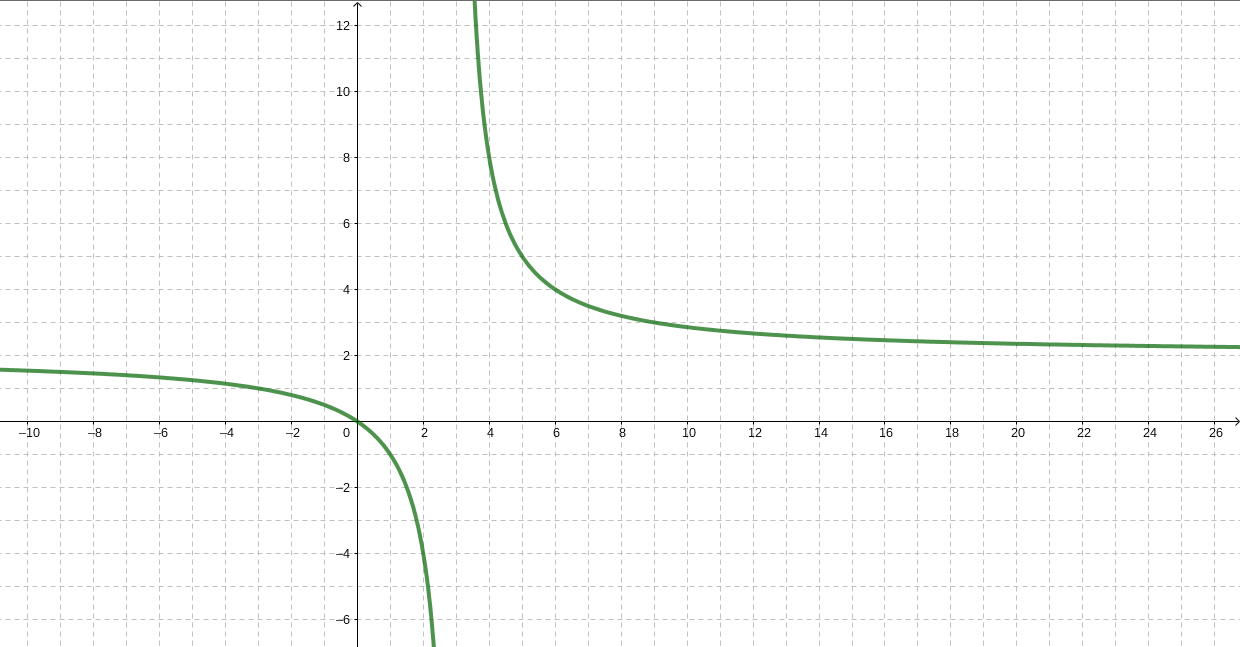
\includegraphics[width=0.9\textwidth]{img/c3r13.png}
        \end{figure}
        
	\end{gabaritoQuestao}
\end{gabarito}

%\end{comment}
\paraTutores

Neste momento, você deve conversar com os estudantes visando orientar tanto o uso de termos adequados (se aproxima, tende a, nunca cruza) quanto a interpretação dos resultados obtidos, pois o gráfico aqui proposto deve ser inédito para a maioria dos estudantes.

%\end{comment}
\paraAmbos
%%É importante que a figura abaixo fique numa pagina diferente da questao anterior
\newpage

O gráfico da função $f(x)=\frac{6}{x-2}+1$ está representado abaixo. Note que ele não corta a reta $y=1$ e não toca a reta $x=2$. Essas retas são chamadas de \textbf{assíntotas} e serão dsicutidas em detalhes pelo seu professor de cálculo.

\begin{figure}[h]
\centering
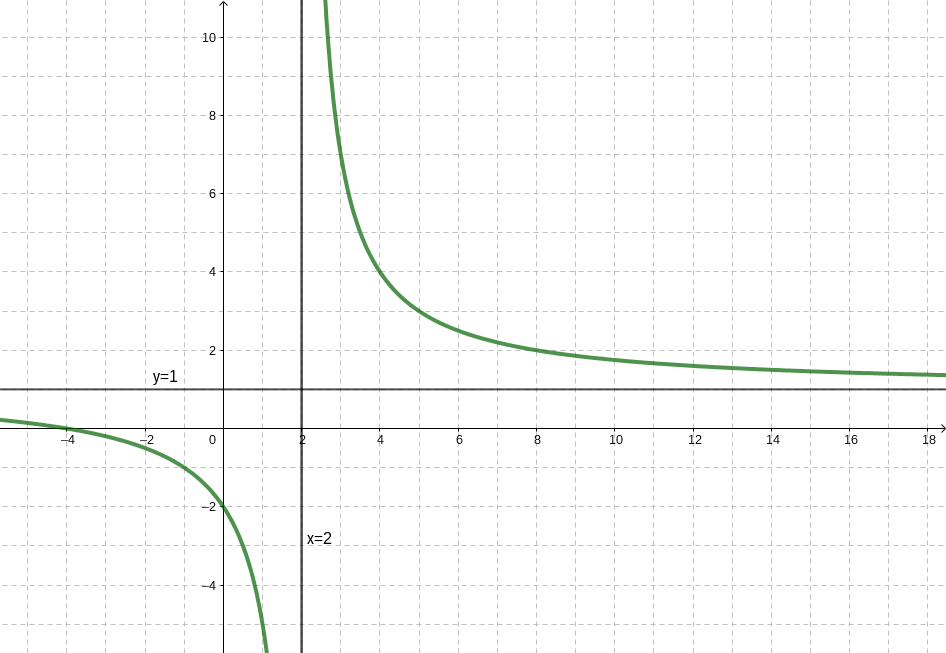
\includegraphics[width=0.4\textwidth]{img/c3q12.png}
\end{figure}

\subsection*{Mais uma função racional}

\begin{questao}
Use a abordagem do bloco anterior para esboçar o gráfico da função $r(x)=\frac{2x}{x-3}$.
\end{questao}
\newpage

%\end{comment}
\paraTutores

Deixe que os estudantes resolvam esta questão por conta própria, mesmo que tome muito tempo. Se estiverem com dificuldade, sugira que voltem e tentem seguir as ideias por trás dos itens das duas questões anteriores.

%\end{comment}
\paraAmbos

\section{Rumo ao livro-texto}

Antes de seguir para a questão abaixo, leia a seção 2.2 do livro \sugestao{Calculus}, de James Stewart, do exemplo 8 até o final do exemplo 9, que segue transcrito abaixo.

\begin{resolvida}
Encontre $lim_{x\rightarrow3^+ \frac{2x}{x-3}}$ e $lim_{x\rightarrow3^- \frac{2x}{x-3}}$.
\end{resolvida}

%\end{comment}
\paraTutores

É importante que os estudantes de fato voltem e leiam a seção sugerida no livro. Afinal, o propósito desta seção é aproximar mais explicitamente o conteúdo abordado neste material ao abordado nas disciplinas regulares. Sem lê-la, os estduantes não conseguirão entender a discussão a seguir.

%\end{comment}
\paraAmbos

Note que essa é a mesma função que você resolveu na última questão antes desta seção. A análise feita no livro conecta as discussão apresentadas aqui com conteúdos que serão explorados de maneira mais formal pelo seu professor de Cálculo.

Como dito no livro, essa função tem uma \textbf{assíntota vertical}, que ocorre quando $x=3$. Para valores de $x$ menores do que 3, a função assume valores negativos cada vez maiores à medida que $x$ se aproxima de $3$. Você pode checar isso calculando o valor da função quando $x=2,9$ e $2,99$. Por outro lado, quando os valores de $x$ são maiores do que $3$, a função assuma valores positivos cada vez maiores à medida que $x$ se aproxima de $3$, como $x=3,1$ e $3,01$.

Além dessa assíntota, e esse aspecto o livro não discutiu, temos uma \textbf{assíntota horizontal} em $y=2$. O gráfico da função nunca toca essa reta, mas se aproxima dela se tomarmos valores de $x$ positivamente muito grandes (como $100$ ou $1000$) ou negativamente muito grandes (como $-100$ ou $-1000$).

A próxima questão, pra você resolver, foi retirada do livro \sugestao{Cálculo}, de James Stewart, seção 2.2.

\begin{resolva}
Considere $f(x)=\frac{x}{x^2-x-2}$.
\begin{enumerate}[a)]
 \item Encontre as assíntotas verticais da função $f(x)$.
 \item Confirme a sua resposta plotando o gráfico da função. \textit{Dica: use o software Geogebra no seu celular, notebook ou PC.}
\end{enumerate}
\end{resolva}

%\end{comment}
\paraTutores

Se houver muito dificuldade, sugira que aos estudantes que testem alguns valores de $x$ e de $y$ e esbocem o gráfico da função manualmente.

%\end{comment}
\paraAmbos

\section{Gabarito}

Confira as respostas para as questões e \textbf{não se esqueça de registrar o seu progresso}.

\imprimeGabarito

%\end{comment}
\paraTutores

\subsection{Questões adicionais}

Para este capítulo, vamos propor apenas uma questão adicional similar as últimas resolvidas pelos estudantes. Porém, se for necessário você pode extrair exemplos e questões para a parte sobre frações algébricas e equações do \href{https://portaldaobmep.impa.br/index.php/modulo/ver?modulo=38}{módulo sobre frações algébricas} do Portal da Matemática.

\begin{adicional}
Esboce o gráfico da função $q(x)=\frac{12}{x^2-7x+10}$.
\end{adicional}

%\end{comment}
\paraAlunos

\section{Auto-avaliação final}
Avalie o quanto você acha que sabe sobre os seguintes itens após ter resolvido as questões deste capítulo.

\begin{center}
 \begin{tabular}{|p{25mm}||p{10mm}|p{10mm}|p{10mm}|p{10mm}|} 
 \hline
   & Nada & Muito pouco & Noções gerais & Muito\\
 \hline
 Fatoração de polinômios &  &  &  &  \\ 
 \hline
 Soma de frações com incógnitas &  &  &  &  \\
 \hline
 Funções racionais &  &  &  &  \\
 \hline
\end{tabular}
\end{center}

Cheque como foi o seu progresso comparando essas respostas com as que você deu antes de estudar este capítulo. Caso você não tenha atingido o nível ``Muito''  em algum dos tópicos acima, liste abaixo qual ação concreta você fará nos próximos dias para atingi-lo:

%\end{comment}
\paraAmbos

\end{document}
